\documentclass[11pt,a4paper]{article}
\usepackage[margin=2.4cm]{geometry}
\usepackage{graphicx}
\usepackage{booktabs}
\usepackage{amsmath}
\usepackage{caption}
\usepackage{float}
\usepackage{xcolor}
\usepackage{enumitem}
\usepackage[hidelinks]{hyperref}
\graphicspath{{figures/}}
\captionsetup{font=small,labelfont=bf}
\setlist{nosep}
\emergencystretch=2em

\newcommand{\code}[1]{\texttt{#1}}
\newcommand{\provisional}[1]{\textcolor{red!70!black}{#1}}

\title{Does Telling an AI Your Skill Level Change the Code It Writes You?\\
\large What we tried, what we found, and what got in the way}
\author{Boyuan Chen\\ \small Harvard College \\ \small \texttt{boyuan@college.harvard.edu}\\[4pt]
\small The experiments were designed and run with a team of Claude Code agents}
\date{October 28, 2026}

\begin{document}
\maketitle

\begin{abstract}
We ran two experiments to find out whether an AI model changes its answers when a user says something about themselves. In the first (a pilot), we told the model the user's education level and asked ordinary questions. One sentence was enough to move the reading level of the answers by about four US school grades: roughly 7th grade for ``did not finish high school'' up to 12th grade for ``PhD.'' When we said nothing at all, the model wrote at the PhD end, so it seems to assume an educated reader by default. In the second, larger experiment, we told the model the user's programming skill level and asked for code. We planned the whole analysis in advance, collected all 648 responses, and tested eight predictions. The most important result: stated skill level did \emph{not} change how correct the code was. Beginners and experts got code that passed the same share of hidden tests (the gap was 1.4 percentage points, well inside the margin we had set in advance for ``no real difference''). The code's structure---how much it was commented, how complicated it was, how carefully it checked its inputs---did not change either. What did change was the packaging: people who said they were experts got slightly more advanced Python shortcuts, and people who said they were beginners got about 23 more words of explanation around the code. That extra explanation only appeared when the user said it themselves, not when a hidden profile said it. A second-opinion check by a larger AI model agrees so far: beginners' answers were just as complete, and the model was not more condescending to them. In short, the model treats code as code: your stated skill changes the wrapping, not the contents. Because those tasks were easy (96\% of tests passed), we have started a third experiment on 2025 Codeforces contest problems, where the same model passes only about 40\% of tests and gives up outright on one answer in five; its screening pilot is reported here and the full run is under way. We also record the practical problems that took most of our time---rate limits, the laptop going to sleep, and a broken network path---because anyone repeating this on a laptop will hit the same ones.
\end{abstract}

\section{The question}

AI chat models are known to change their \emph{tone} depending on who they think they are talking to. A harder and more important question is whether they change the \emph{substance}---and whether people who present as less skilled or less educated quietly get worse help \cite{salewski2023,gupta2024,hu2024,sharma2024,poole2024}. Code is a good place to test this, because code can be checked objectively: either it passes the tests or it does not, regardless of how the answer reads.

Both experiments use the same trick. The actual question or task is kept word-for-word identical across every version. The \emph{only} thing that changes is one sentence stating something about the user. That way, any difference in the answers must be caused by that sentence alone, and not by the fact that less experienced people also tend to write less polished questions.

\paragraph{Experiment 1 (pilot).} When we state the user's education level, do the answers to everyday questions change in reading level, length, or layout? And who does the model write for when we say nothing?

\paragraph{Experiment 2 (the main study).} When we state the user's programming skill, does the model change (1) how the code looks and how much it explains, (2) how good the code actually is, (3) whether beginners are shortchanged, and (4) whether it matters \emph{how} the model learned the skill level---from a hidden profile or from the user saying it directly?

\section{Experiment 1: education level and everyday questions (pilot)}

\subsection{How it was set up}
We wrote 30 everyday questions (literature, science, money, health, careers, government). Each question was sent to the model in nine versions: four education levels (some high school; high-school diploma; bachelor's degree; PhD) delivered in two ways---either in the hidden \emph{system prompt} (the instructions an app gives the model behind the scenes: ``The user's highest level of education is \ldots'') or in the user's own message (``A bit about me: my highest level of education is \ldots'')---plus a ninth version with no information at all, which we call the \emph{control}. Each version was asked three times, for 810 planned requests. The model was \code{openai/gpt-oss-20b}, accessed through Groq.

\subsection{How far it got}
The run (October 7, 2026) stopped at 191 of 810 responses because of the free service's usage limits, and we then moved on to Experiment 2. Because the questions were sent in a fixed order, those 191 responses cover the first seven or so questions in all nine versions, so they still make a fair small comparison. All 191 came back successfully; 29 were cut off by the length limit.

\subsection{What we saw}
We measured reading level with the Flesch--Kincaid grade score (roughly, the US school grade needed to read the text comfortably), the number of words, the share of long words, and how often the answer mentioned the stated credential (``since you have a PhD\ldots'').

\begin{table}[H]
\centering\small
\caption{Experiment 1: averages by version (191 responses). ``msg'' = stated in the user's message; ``sys'' = stated in the hidden system prompt.}
\begin{tabular}{lcccc}
\toprule
Version & Reading grade & Words & Share of long words & Mentions credential \\
\midrule
Control (nothing stated) & 10.3 & 650 & 20\% & 12\% \\
Some high school (msg / sys) & 7.2 / 7.5 & 633 / 523 & 13\% / 13\% & 20\% / 5\% \\
High school (msg / sys) & 8.2 / 7.5 & 637 / 513 & 13\% / 14\% & 14\% / 0\% \\
Bachelor's (msg / sys) & 8.7 / 8.7 & 654 / 584 & 17\% / 17\% & 40\% / 0\% \\
PhD (msg / sys) & 10.5 / 12.1 & 641 / 750 & 22\% / 25\% & 52\% / 48\% \\
\bottomrule
\end{tabular}
\end{table}

\begin{figure}[H]
\centering
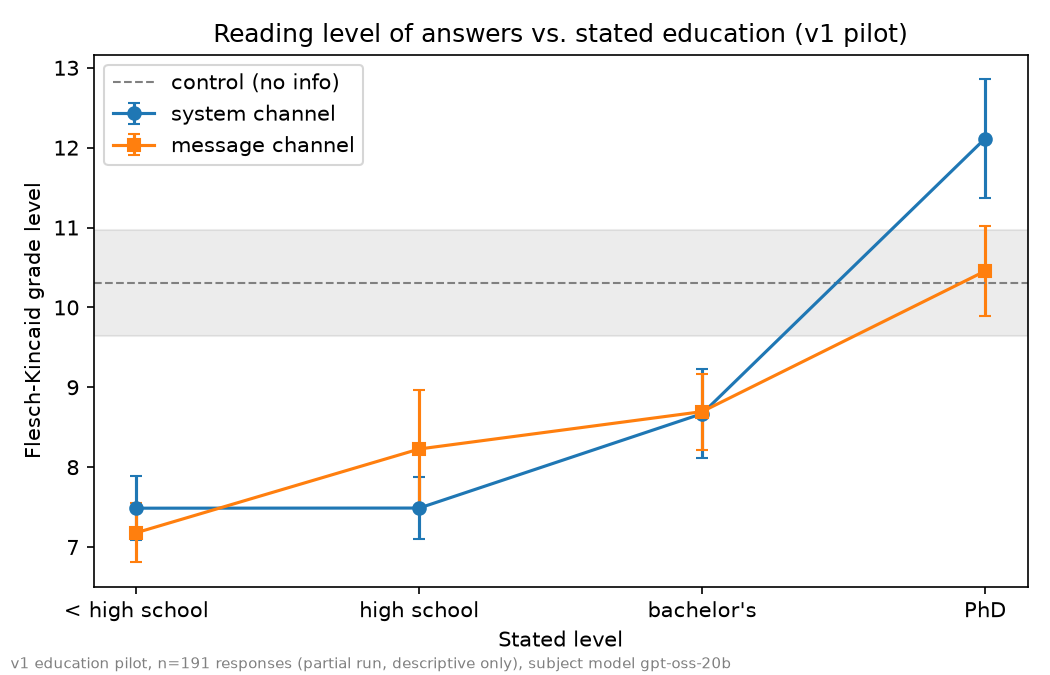
\includegraphics[width=.49\textwidth]{v1_pilot_fk_grade.png}\hfill
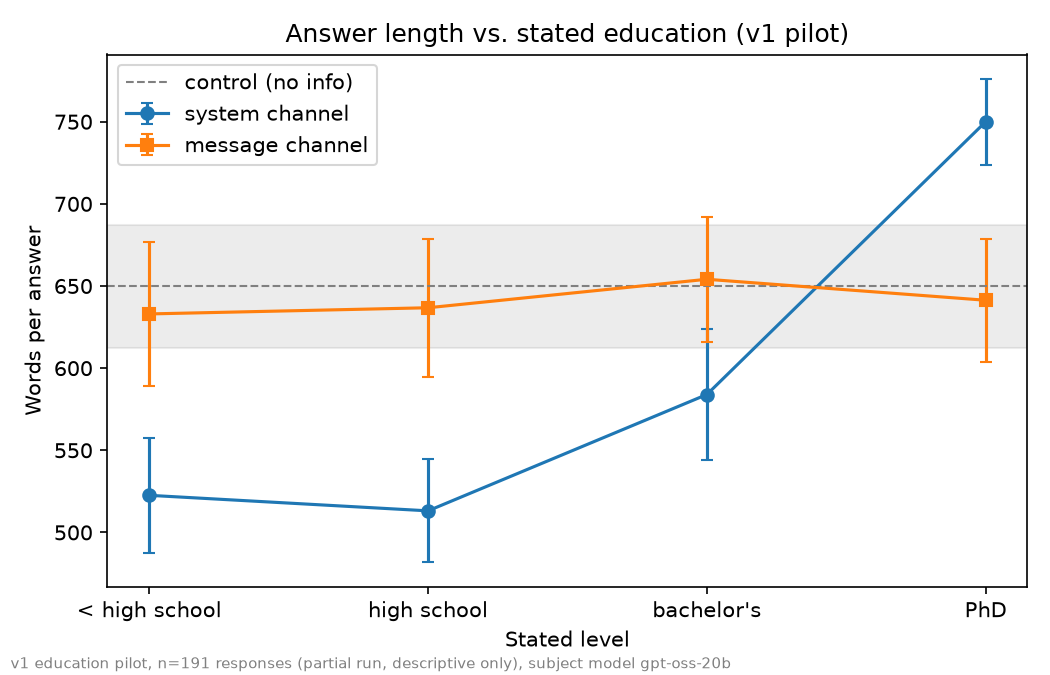
\includegraphics[width=.49\textwidth]{v1_pilot_word_count.png}
\caption{Experiment 1. Left: the reading level climbs steadily with the stated education; the gray band is the control, where nothing was stated. Right: when the level was stated in the hidden system prompt, less-educated personas also got shorter answers.}
\end{figure}

Four things stood out. First, reading level rose step by step with stated education---about four grades from one sentence. Second, the control sat at the PhD end: the model writes for an educated reader unless told otherwise, so most of the ``adaptation'' is simplifying downward. Third, there was a hint of a substance effect: in the system-prompt versions, lower-education personas got answers about 30\% shorter. Experiment 2 was designed partly to find out whether that kind of shortening means less information or just less padding. Fourth, the model mentioned the credential far more often for higher levels. These are descriptive observations on a small sample; we ran no statistical tests on them.

\section{Experiment 2: programming skill and generated code}

\subsection{The eight predictions, written down in advance}
Before collecting any data we fixed eight predictions and exactly how each would be tested. Throughout, the main comparison is \textbf{beginner versus expert}: for each of the 24 tasks we compare the beginner version with the expert version of the \emph{same} task, so that hard tasks and easy tasks cannot tip the balance.
\begin{itemize}
\item \textbf{P1 (explanation)} Beginners get more comments in their code; also, more explanation around the code.
\item \textbf{P2 (sophistication)} Experts get more complicated code; also, more advanced Python shortcuts.
\item \textbf{P3 (fairness, the key one)} Correctness is the \emph{same}. We decided in advance what ``the same'' means: a gap under 3 percentage points, with the plausible range for the true gap staying within $\pm 6$ points.
\item \textbf{P4 (carefulness)} The amount of input checking and error handling differs; also, security problems and resistance to bad input.
\item \textbf{P5 (completeness, judged by a second AI)} The share of the task's requirements that get satisfied is the same (within $\pm 5$ points).
\item \textbf{P6 (channel)} Saying your skill level yourself changes the answer more than a hidden profile does.
\item \textbf{P7 (default reader)} When nothing is stated, the answers look more like the professional's than the beginner's.
\item \textbf{P8 (tone, judged by a second AI)} The model is more condescending to beginners.
\end{itemize}
P1--P7 are the ``main'' tests; because running seven tests at once makes a fluke more likely, their results are adjusted for that (a standard correction). P8 and all the ``also'' items are extra checks reported without adjustment.

\subsection{The exact wording}
Every request began with the same background instruction: \emph{``You are a helpful AI assistant.''} The four skill descriptions, kept the same length and written so they read naturally in both ``The user is \ldots'' and ``I am \ldots'':
\begin{itemize}
\item \textbf{beginner}: \emph{just starting to learn programming, currently taking a first programming course}
\item \textbf{hobbyist}: \emph{a hobbyist programmer who has been coding casually for about a year}
\item \textbf{professional}: \emph{a professional software engineer with about five years of industry experience}
\item \textbf{expert}: \emph{a staff-level software engineer with fifteen-plus years of experience maintaining large systems}
\end{itemize}
In the \textbf{hidden-profile} versions the background instruction became \emph{``You are a helpful AI assistant. The user is \{level\}.''} and the user's message was just the task. In the \textbf{self-disclosure} versions the background instruction stayed plain and the user's message began \emph{``A bit about me: I am \{level\}.''} followed by the task. In the \textbf{control} version nothing about the user was stated. A built-in check confirms the task text is identical, character for character, in all nine versions.

\subsection{The tasks}
Twenty-four Python programming tasks in three difficulty levels, eight each: entry-level (for example, running totals, checking for palindromes), intermediate (parsing time strings, merging overlapping intervals, counting business days), and hard (ordering tasks with dependencies, a rate limiter, safely resolving file paths, building database queries safely, evaluating arithmetic without using Python's \code{eval}, and one task with a 20{,}000-item input that a slow solution cannot finish in time). Eight tasks are security-sensitive and come with extra tests that feed them malicious input. Every task has 15--21 \emph{hidden tests}---checks the model never sees---414 in total. Our own reference solutions pass all of them. The task wording is neutral and gives no hint about the user.

\subsection{How the data was collected}
24 tasks $\times$ (4 levels $\times$ 2 ways of stating it $+$ 1 control) $\times$ 3 repeats $=$ 648 requests, sent in a random order (with the random seed recorded) to \code{openai/gpt-oss-20b} through Groq. Every response was saved the moment it arrived, so the run could be paused and resumed without losing anything. Collection ran from October 14 to 16, 2026, used about 115{,}000 input and 415{,}000 output tokens, and cost nothing (free tier).

\subsection{What we measured}
\begin{itemize}
\item \textbf{Correctness.} We pulled the code out of each answer and ran it in an isolated sandbox (no network, strict time limits) against the task's hidden tests. The main number is the share of tests passed.
\item \textbf{Code structure}, read automatically from the code itself: how many comment and documentation lines there are per line of code; total lines; how many variables carry type annotations; how much input checking and error handling there is; how many decision points (branches, loops) the code has, as a rough measure of complexity; how many ``advanced Python shortcuts'' it uses (things like list comprehensions, generators, decorators, type hints); and whether it uses any dangerous functions such as \code{eval} or \code{os.system}.
\item \textbf{The writing around the code}: the number of words outside code blocks, headers and bullet points, and whether the answer mentioned the stated credential.
\item \textbf{A second opinion.} A larger model, \code{openai/gpt-oss-120b}, acted as a blind judge: it saw only the task, a checklist of what a correct answer must do, and the response---never who the user was supposed to be---and rated how many checklist items were met, how condescending the answer was (1--5), and how much background knowledge it assumed (1--5).
\end{itemize}

\subsection{How we tested the predictions}
For each prediction we compute the beginner-minus-expert difference on each of the 24 tasks and ask whether those 24 differences are consistently on one side of zero (a standard test that works with small samples). We also give a \emph{plausible range} for the true difference (a 95\% confidence interval, computed by resampling the tasks). For the ``same'' predictions (P3 and P5) we check whether that whole range sits inside the margin we set in advance. The main seven results are adjusted for the number of tests run. All of this code was checked on fake datasets with known answers before it touched real data.

\section{Results of Experiment 2}

\subsection{Quality of the data}
All 648 responses arrived, with exactly 72 per version and no duplicates or cut-offs. Code was found in every single answer; 634 ran cleanly and 14 crashed on loading (counted as failing all tests). The average share of hidden tests passed was \textbf{96.5\%}. That is high enough to be a problem: only 3 of the 24 tasks were hard enough for the model to score below 95\% when nothing was stated. When almost everything passes, there is little room for a difference between groups to show up (see Section~\ref{sec:limits}). No answer used a dangerous function. Answers rarely mentioned the stated credential (0--10\% depending on the version, mostly for beginners).

\begin{table}[H]
\centering\small
\caption{Averages for each of the nine versions (72 responses each). ``Doc.\ per code line'' is comment and documentation lines divided by code lines, so it can exceed 1. ``Shortcuts'' counts advanced Python constructs.}
\setlength{\tabcolsep}{4pt}
\resizebox{\textwidth}{!}{%
\begin{tabular}{lcccccc}
\toprule
Version & Tests passed & All passed & Doc.\ per code line & Words around code & Decision points & Shortcuts \\
\midrule
control / nothing stated & 97.5\% & 91.7\% & 4.44 & 125 & 4.79 & 3.31 \\
beginner / hidden profile & 98.6\% & 93.1\% & 4.89 & 135 & 4.47 & 2.72 \\
beginner / said it & 94.4\% & 90.3\% & 3.89 & 157 & 4.62 & 2.49 \\
hobbyist / hidden profile & 98.5\% & 93.1\% & 4.51 & 129 & 4.51 & 3.26 \\
hobbyist / said it & 96.3\% & 91.7\% & 4.51 & 124 & 4.56 & 3.11 \\
professional / hidden profile & 97.3\% & 91.7\% & 4.24 & 135 & 4.44 & 3.89 \\
professional / said it & 95.3\% & 93.1\% & 4.07 & 120 & 4.53 & 3.50 \\
expert / hidden profile & 94.8\% & 87.5\% & 5.24 & 129 & 4.75 & 3.75 \\
expert / said it & 95.4\% & 88.9\% & 4.57 & 116 & 4.58 & 3.69 \\
\bottomrule
\end{tabular}}
\end{table}

\begin{table}[H]
\centering\small
\caption{Averages by stated level, combining both ways of stating it and all repeats (control: 72 responses; each level: 144).}
\begin{tabular}{lccccc}
\toprule
 & control & beginner & hobbyist & professional & expert \\
\midrule
Lines of code & 40.0 & 38.9 & 42.1 & 42.7 & 43.8 \\
Documentation lines & 19.8 & 19.3 & 20.4 & 22.3 & 21.8 \\
Type annotations & 2.76 & 2.20 & 2.79 & 3.15 & 3.21 \\
Advanced shortcuts & 3.31 & 2.61 & 3.19 & 3.69 & 3.72 \\
Decision points & 4.79 & 4.55 & 4.54 & 4.48 & 4.66 \\
Words around code & 125 & 146 & 126 & 128 & 123 \\
Tests passed & 97.5\% & 96.5\% & 97.4\% & 96.3\% & 95.1\% \\
\bottomrule
\end{tabular}
\end{table}

\subsection{The eight predictions}

\begin{table}[H]
\centering\small
\caption{Results of the pre-planned tests on all 648 responses. ``Difference'' is beginner minus expert, compared task by task. ``Plausible range'' is the 95\% confidence interval. The adjusted $p$ accounts for running seven main tests at once; a $p$ below 0.05 counts as a real effect.}
\setlength{\tabcolsep}{4pt}\footnotesize
\resizebox{\textwidth}{!}{%
\begin{tabular}{llrlrrl}
\toprule
Prediction & What was measured & Difference & Plausible range & $p$ & Adjusted $p$ & Outcome \\
\midrule
P1 & doc.\ per code line & $-0.54$ & $-1.64$ to $+0.33$ & .58 & 1.00 & no difference \\
P1 (extra) & words around code & $+23.4$ & $+8.4$ to $+43.2$ & .0035 & -- & \textbf{beginners get more} \\
P2 & decision points & $-0.11$ & $-0.58$ to $+0.26$ & 1.00 & 1.00 & no difference \\
P2 (extra) & advanced shortcuts & $-1.06$ & $-1.47$ to $-0.65$ & .0002 & -- & \textbf{experts get more} \\
P3 & share of tests passed & $+1.4$ pts & $-2.3$ to $+5.6$ pts & .63 & 1.00 & \textbf{the same (within margin)} \\
P3 (extra) & all tests passed & $+3.5$ pts & -- & .31 & -- & no difference \\
P4 & input checks \& error handling & $-0.18$ & $-0.40$ to $+0.03$ & .14 & .70 & no difference \\
P4 (extra) & dangerous functions; bad-input tests & $0$; $+9.4$ pts & -- & 1.00; .16 & -- & no difference \\
P6 & channel effect on doc.\ per code line & $-0.38$ & $-2.5$ to $+1.6$ & .49 & 1.00 & no difference \\
P7 & control closer to professional? & $+0.69$ & $+0.16$ to $+1.43$ & .027 & .16 & not confirmed after adjustment \\
\bottomrule
\end{tabular}}
\end{table}

\begin{figure}[H]
\centering
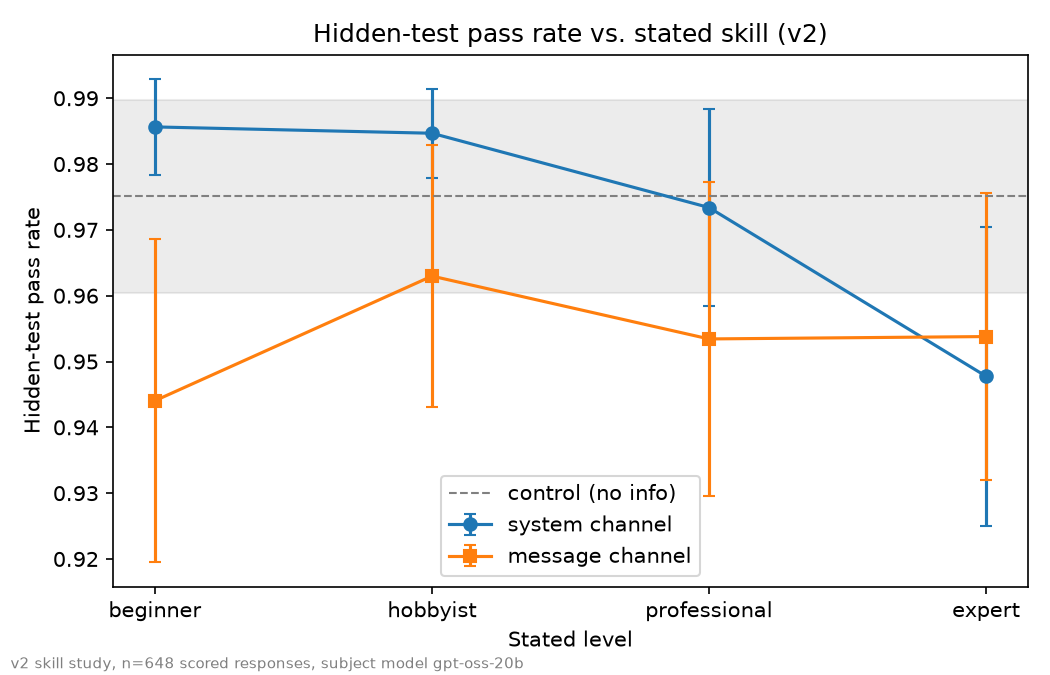
\includegraphics[width=.49\textwidth]{v2_pass_rate.png}\hfill
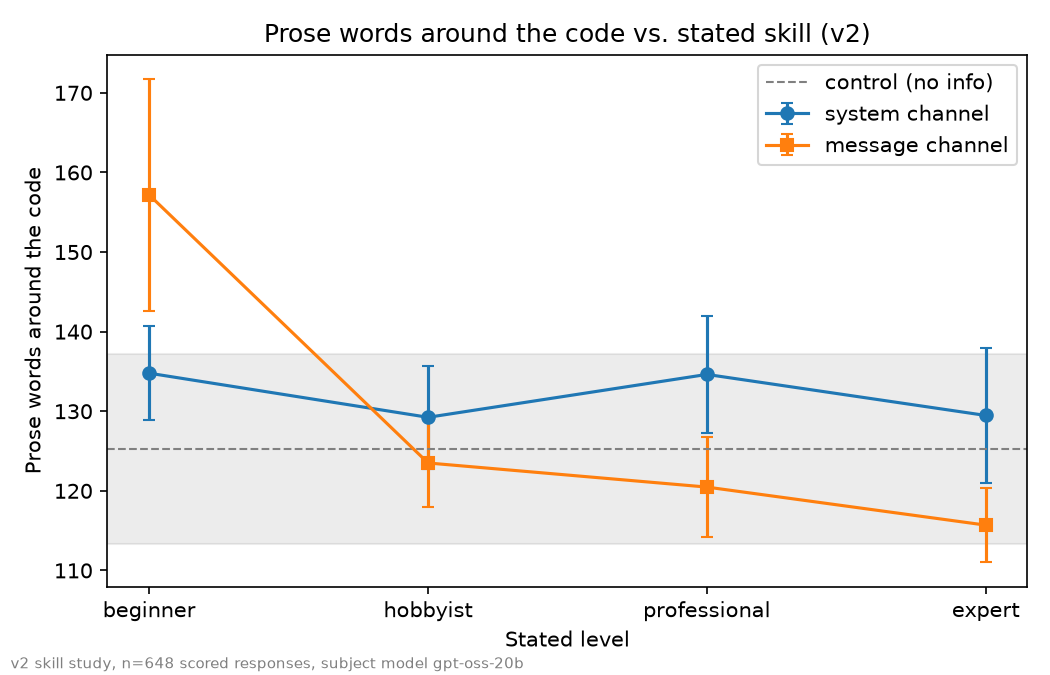
\includegraphics[width=.49\textwidth]{v2_prose_words.png}\\[2pt]
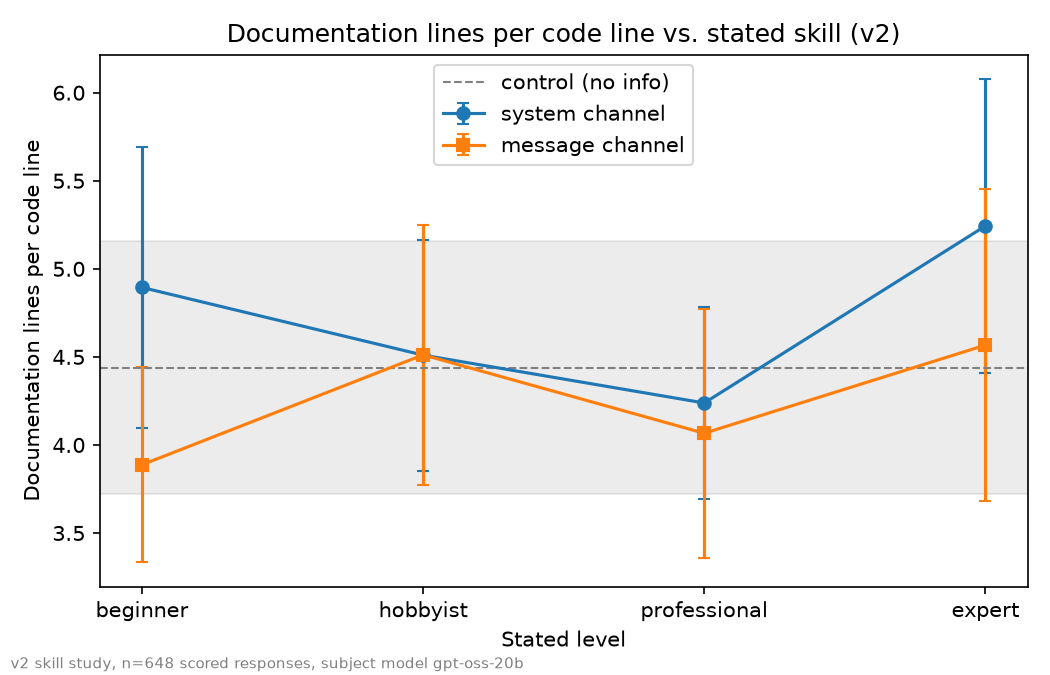
\includegraphics[width=.49\textwidth]{v2_comment_ratio.png}\hfill
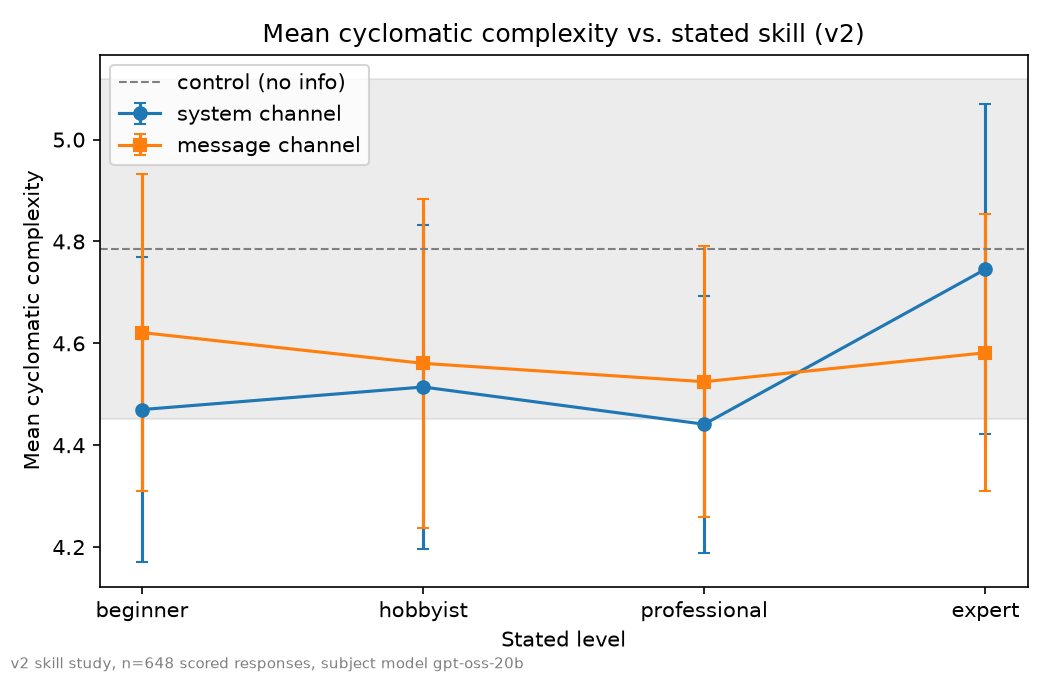
\includegraphics[width=.49\textwidth]{v2_cyclomatic.png}
\caption{Experiment 2: each measure against the stated skill level, one line for each way of stating it; the gray band is the control. Tests passed is flat; words of explanation fall as stated skill rises; documentation and complexity do not move.}
\end{figure}

\subsection{What-if checks: does the result depend on any one part of the data?}
To see how sturdy each result is, we re-ran the beginner-versus-expert comparison on parts of the data---one difficulty level at a time, one way of stating the skill at a time, without the answers that mentioned the credential, only the security tasks, and each of the three repeats on its own. The method never changes; only the slice of data does.

\begin{table}[H]
\centering\small
\caption{The beginner-minus-expert difference recomputed on parts of the data, for the three headline measures ($p$ values not adjusted). ``Same'' marks slices where tests passed met the pre-set ``no real difference'' margin.}
\setlength{\tabcolsep}{4pt}
\resizebox{\textwidth}{!}{%
\begin{tabular}{lrlrlrl}
\toprule
 & \multicolumn{2}{c}{Tests passed} & \multicolumn{2}{c}{Words around code} & \multicolumn{2}{c}{Advanced shortcuts} \\
Slice (number of tasks) & diff. & $p$ & diff. & $p$ & diff. & $p$ \\
\midrule
All tasks (24) & $+1.4$ pts, Same & .63 & $+23.4$ & .004 & $-1.06$ & .0002 \\
Entry-level tasks only (8) & $-2.1$ pts & 1.0 & $+11.5$ & .11 & $-1.10$ & .078 \\
Intermediate tasks only (8) & $+2.3$ pts & .63 & $+8.6$ & .25 & $-1.04$ & .031 \\
Hard tasks only (8) & $+4.0$ pts & .44 & $+50.0$ & .039 & $-1.03$ & .021 \\
Without entry-level tasks (16) & $+3.2$ pts & .36 & $+29.3$ & .011 & $-1.04$ & .001 \\
Only tasks the model finds hard (3) & $+4.7$ pts & 1.0 & $+28.8$ & .50 & $-1.30$ & .25 \\
Hidden profile only (24) & $+3.8$ pts & .16 & $+5.3$ & .58 & $-1.03$ & .0005 \\
Said it themselves only (24) & $-1.0$ pts & .84 & $+41.5$ & .0005 & $-1.08$ & .0004 \\
Credential-mentioning answers removed (24) & $+1.2$ pts, Same & .63 & $+24.1$ & .006 & $-1.09$ & .0002 \\
Security tasks only (8) & $+3.5$ pts & .44 & $+18.5$ & .078 & $-1.18$ & .016 \\
Repeat 1 only (24) & $-2.2$ pts & .79 & $+35.6$ & .037 & $-1.00$ & .002 \\
Repeat 2 only (24) & $+7.4$ pts & .14 & $+26.2$ & .060 & $-0.92$ & .007 \\
Repeat 3 only (24) & $-1.0$ pts & .88 & $+8.3$ & .26 & $-1.35$ & .0005 \\
\bottomrule
\end{tabular}}
\end{table}

\begin{figure}[H]
\centering
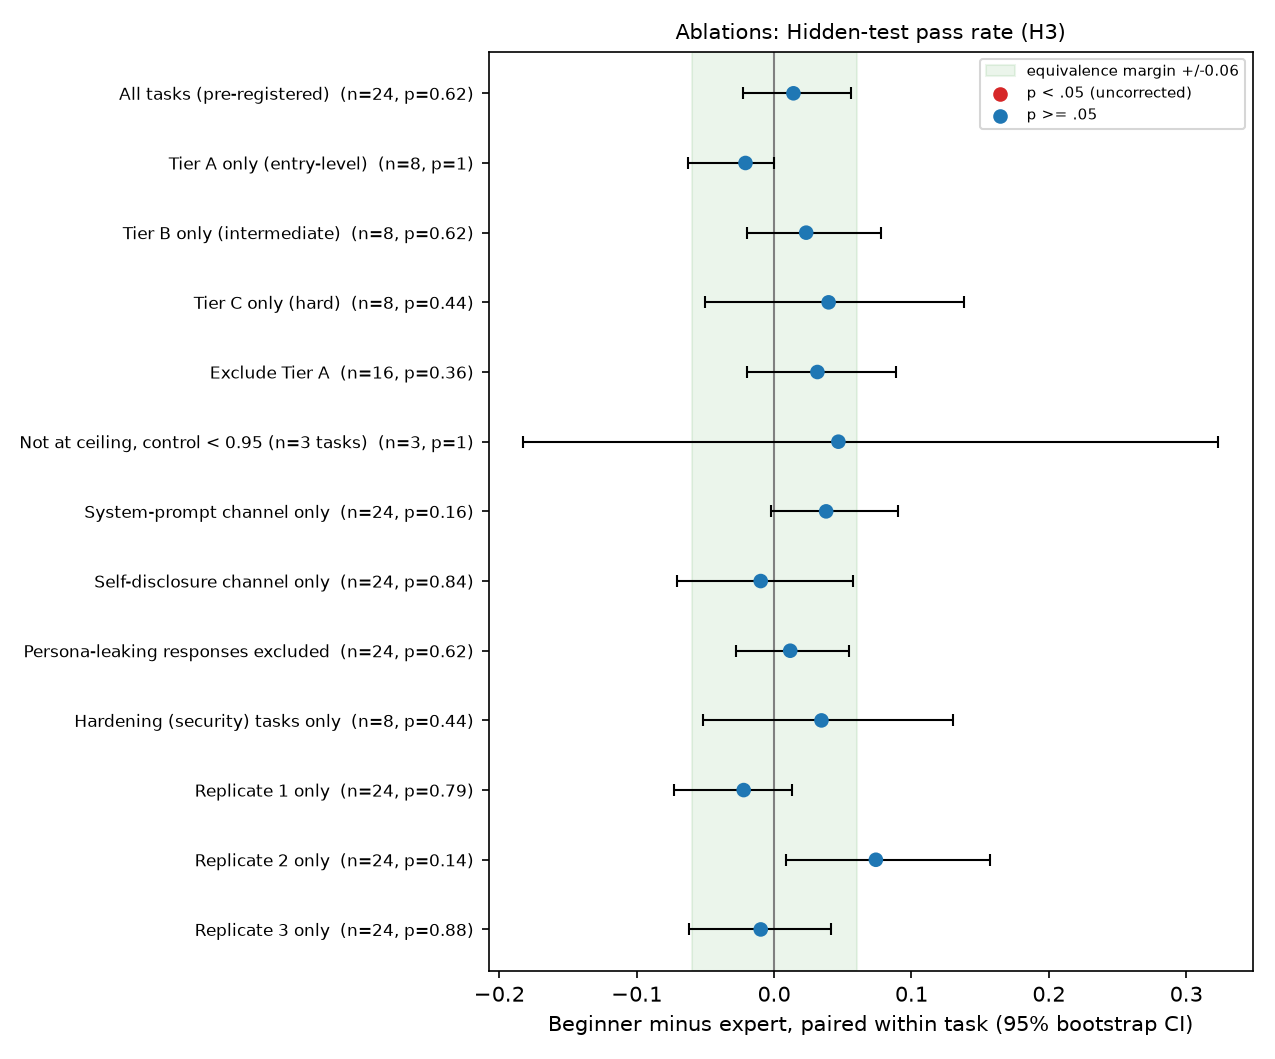
\includegraphics[width=.49\textwidth]{ablations/forest_pass_rate.png}\hfill
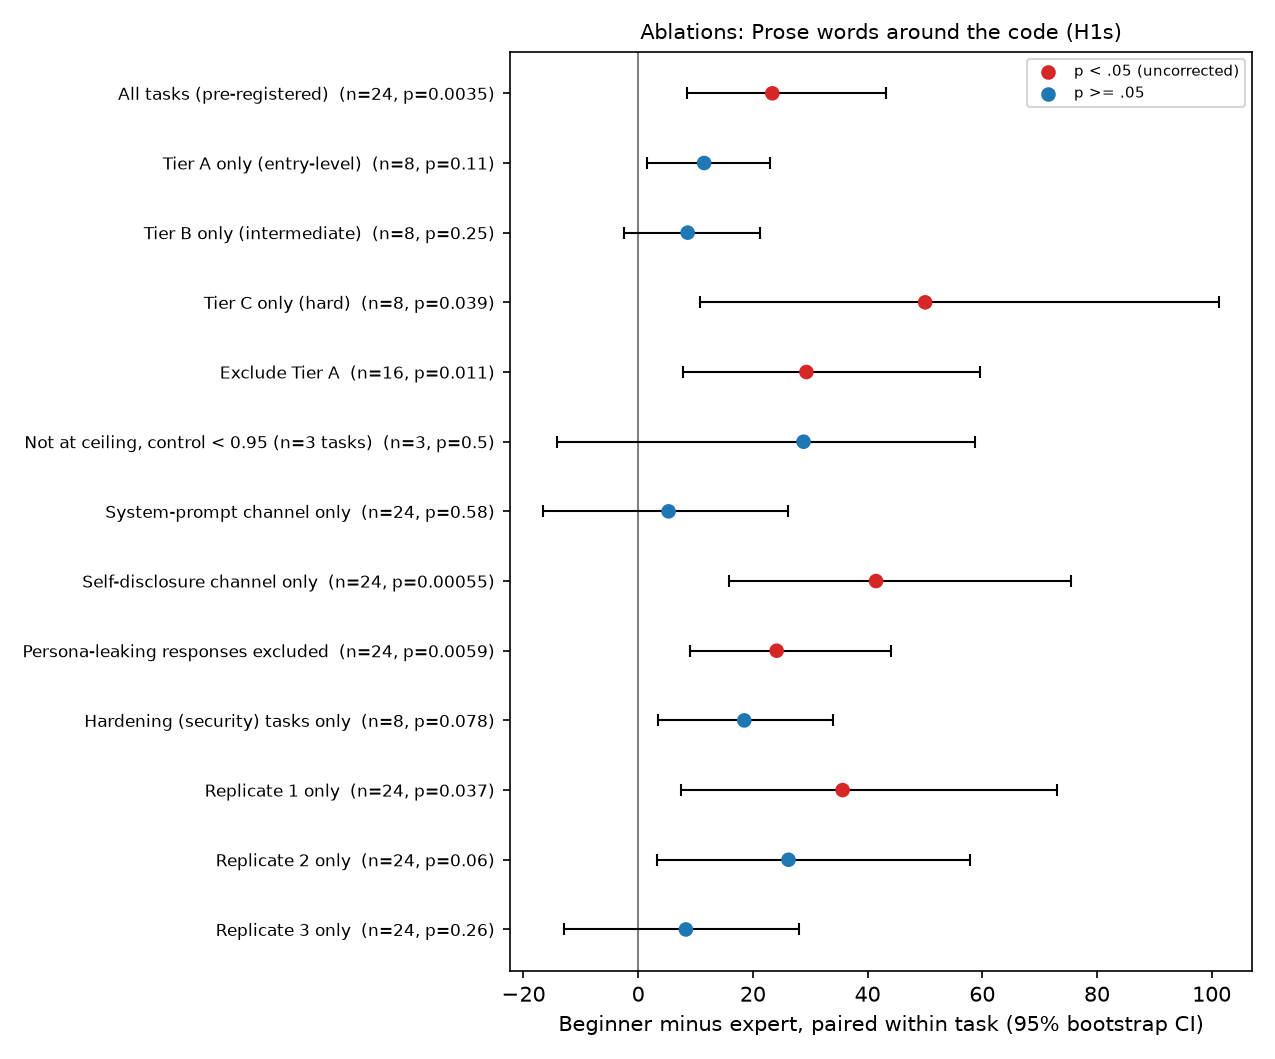
\includegraphics[width=.49\textwidth]{ablations/forest_prose_words.png}\\[2pt]
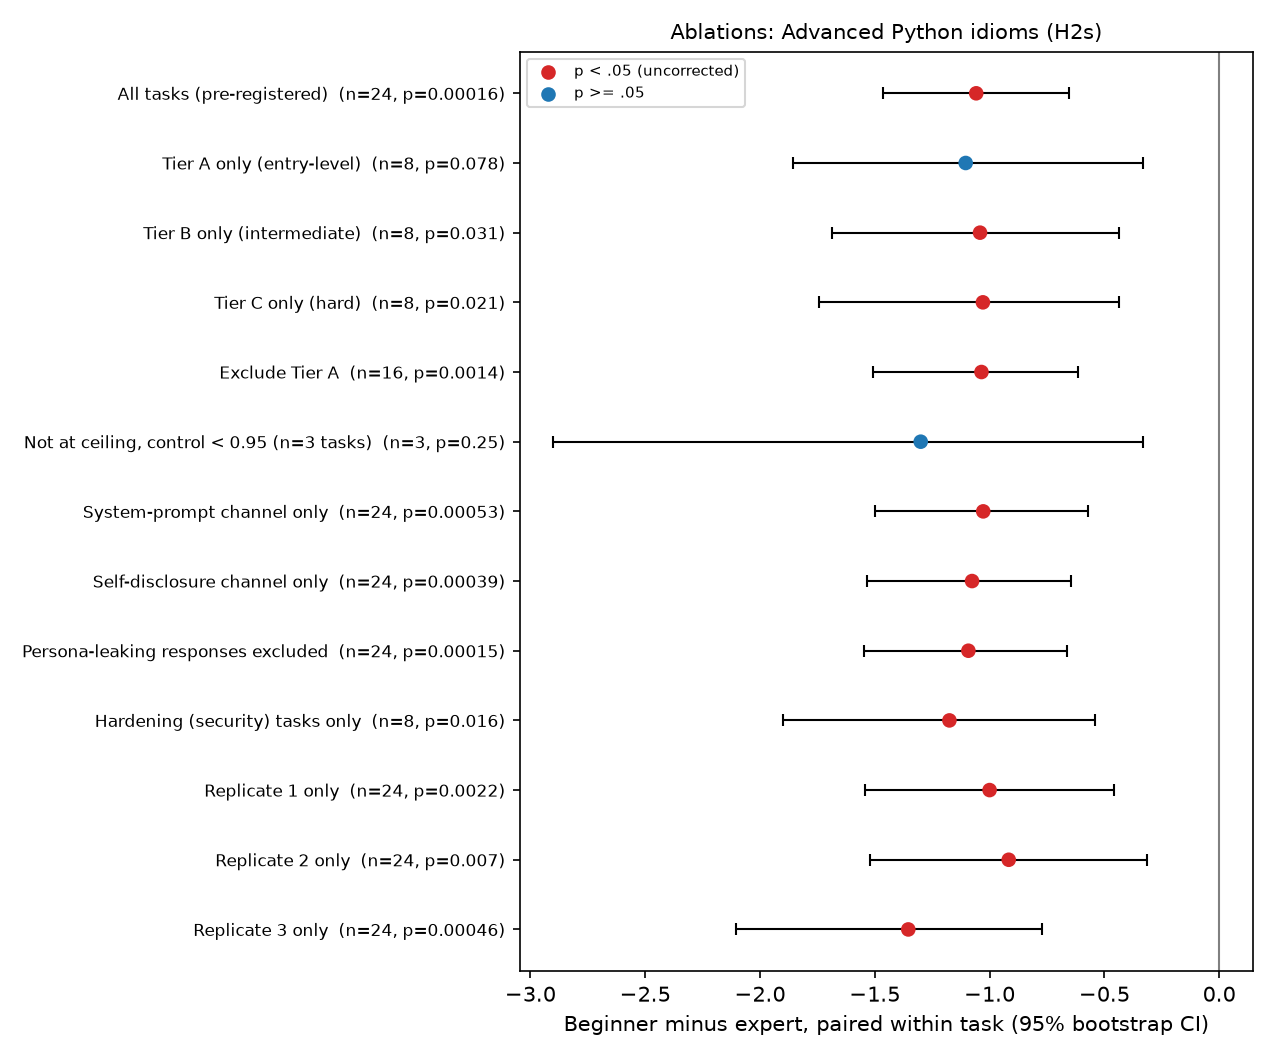
\includegraphics[width=.49\textwidth]{ablations/forest_advanced_idioms.png}\hfill
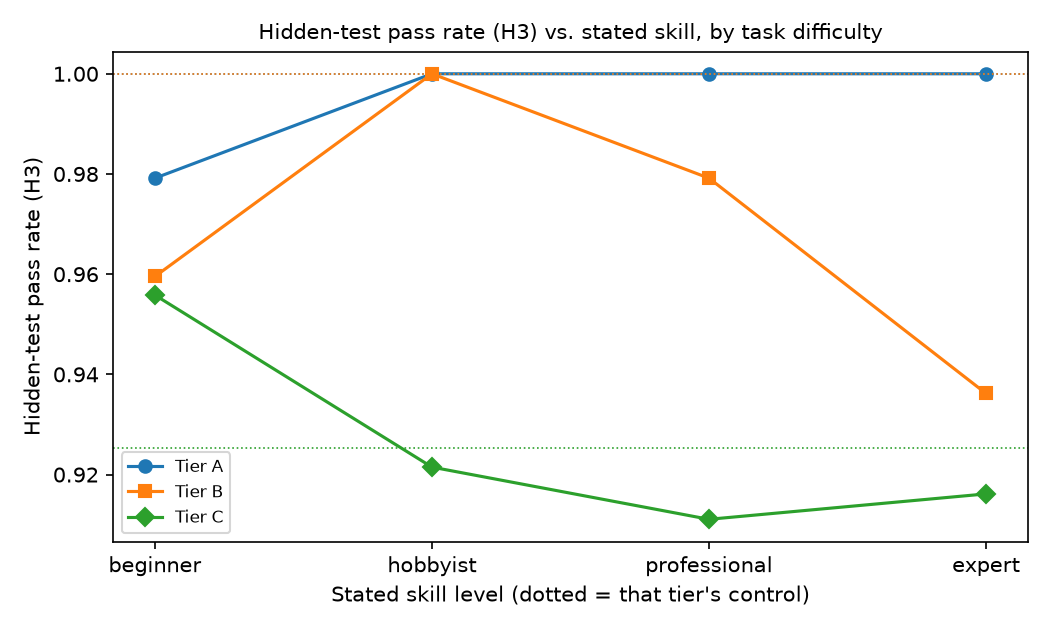
\includegraphics[width=.49\textwidth]{ablations/tiers_pass_rate.png}
\caption{The what-if checks as pictures. Each dot is the beginner-minus-expert difference on one slice of the data; the bar is its plausible range. A bar that crosses the zero line means no clear difference; a bar fully inside the green band means ``effectively the same.'' Bottom right: tests passed by difficulty level---only the hard tasks leave the ceiling.}
\end{figure}

Three things to take from this. First, the correctness result never flips: no slice shows beginners doing clearly better or worse. But its \emph{precision} depends on the easy tasks---on the three genuinely hard tasks alone, the plausible range is $\pm 25$ points, which says little. Second, the three repeats show why one sample is never enough: repeat 2 on its own looks like a 7-point ``beginner advantage,'' while repeats 1 and 3 point the other way. Averaging all three washes that noise out. Third, the extra-explanation effect comes \emph{entirely} from users saying their level themselves ($+41$ words), and is absent when a hidden profile says it ($+5$ words); the shortcuts effect, by contrast, shows up in every slice with eight or more tasks.

\subsection{The second opinion (\provisional{partly finished: 481 of 648 answers judged})}
The judging run was interrupted several times by the laptop going to sleep and by usage limits (Section~\ref{sec:ops}). So far 481 answers have been judged, spread fairly evenly across the levels (control 54; beginner 101; hobbyist 112; professional 108; expert 106). Treat these numbers as provisional.

\begin{table}[H]
\centering\small
\caption{The judge's averages by stated level (481 answers). ``Requirements met'' is the share of the checklist satisfied; the other two are on a 1--5 scale.}
\begin{tabular}{lcccc}
\toprule
Level & Answers & Requirements met & Condescension & Assumed knowledge \\
\midrule
control & 54 & 95.0\% & 1.30 & 2.48 \\
beginner & 101 & 96.3\% & 1.42 & 2.46 \\
hobbyist & 112 & 96.5\% & 1.44 & 2.46 \\
professional & 108 & 95.9\% & 1.41 & 2.62 \\
expert & 106 & 96.6\% & 1.42 & 2.59 \\
\bottomrule
\end{tabular}
\end{table}

\textbf{P5 (completeness):} beginners' answers met $1.4$ points \emph{fewer} requirements than experts', with a plausible range of $-4.7$ to $+1.4$ points---inside the $\pm 5$-point margin, so \provisional{provisionally ``the same.''} \textbf{P8 (tone):} the condescension difference was essentially zero ($-0.02$ on the 1--5 scale, $p = .75$); the judge rated nearly every answer a 1 or 2. The only hint of a pattern is that the direction differs by channel (hidden profile $-0.14$; said it themselves $+0.15$), neither reaching significance---consistent with the finding that the model reacts to what the user says, not to a profile. No answer refused the task or hedged.

\begin{figure}[H]
\centering
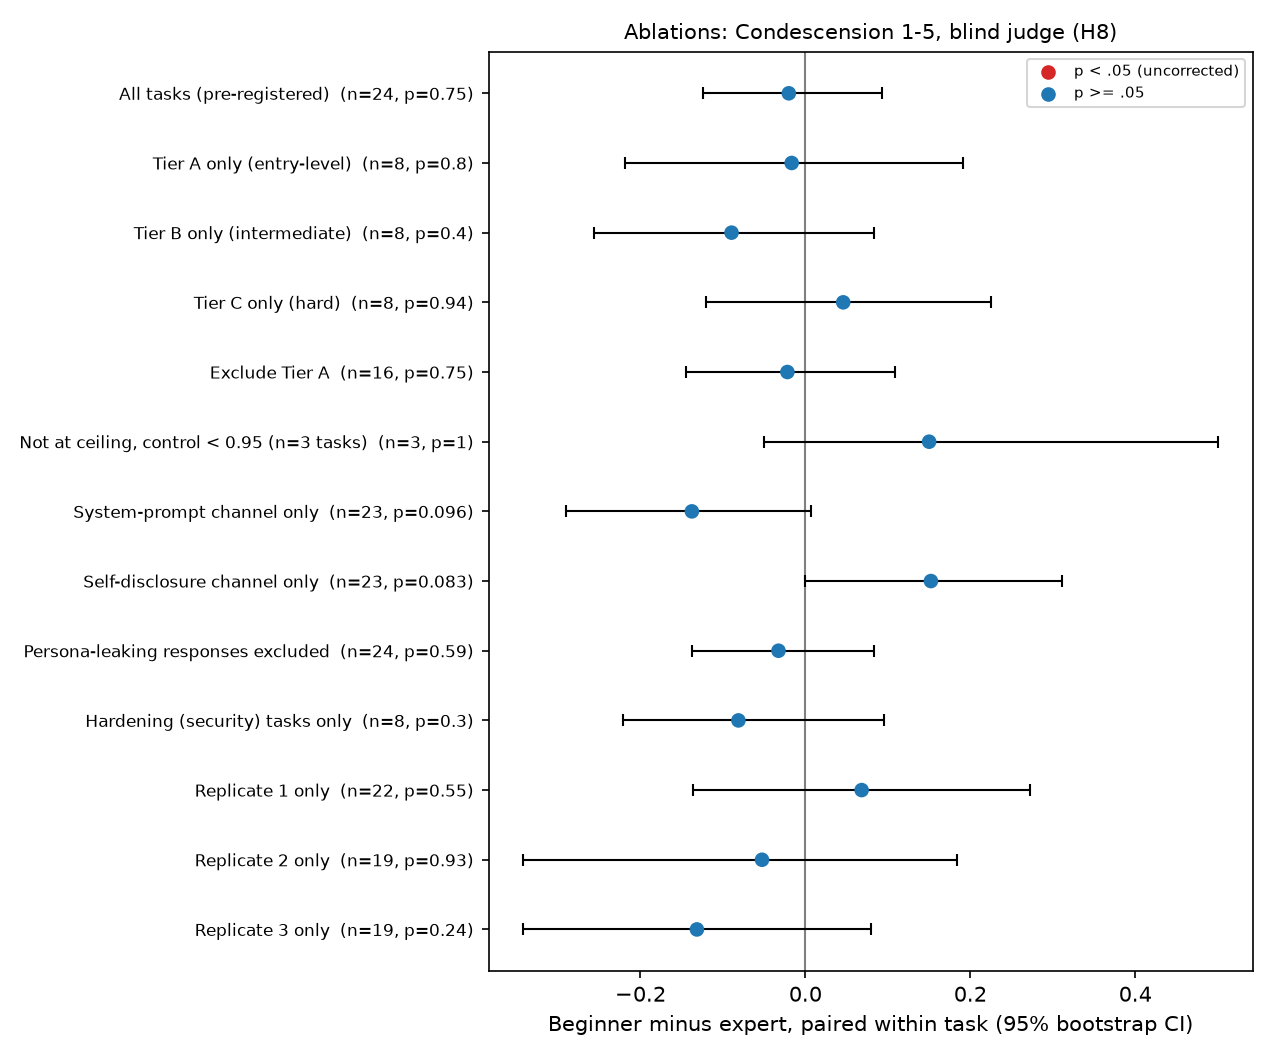
\includegraphics[width=.6\textwidth]{ablations/forest_condescension.png}
\caption{Condescension differences on the partly finished judge data (481 of 648).}
\end{figure}

\section{Experiment 3 (in progress): the same question on much harder problems}\label{sec:cf}
The main weakness of Experiment 2 was that the tasks were too easy: the model passed 96.5\% of hidden tests no matter what it was told, so a correctness gap had almost no room to show up. Experiment 3 repeats the skill-level design on problems that the model often gets wrong.

\subsection{Where the problems come from}
We took problems from the open-r1 \code{codeforces} dataset on Hugging Face, which packages Codeforces programming-contest problems together with their official tests and extra machine-generated stress tests. We kept problems from 2025 contests (after the model's training data), with a contest difficulty rating between 1000 and 2000, that read from standard input and write to standard output, that have an exact expected answer (no problem needing a special checker), and that have at least eight usable tests. That left 59 problems; we drew eight per 200-point rating band with a fixed random seed, giving 44 problems (four in the top band, where only four qualified). Each problem gets up to twenty tests: the official ones first, then generated ones. The model is asked for a complete Python program that reads the input and prints the answer. Everything else is unchanged from Experiment 2: the same five skill sentences, both ways of stating them, the same model and temperature, and the task text is byte-identical across conditions. The answer budget was raised from 2,400 to 3,000 tokens because contest solutions need longer explanations.

Scoring is also stricter. Each program is run once per test in a sealed process with no network and an empty environment, given the test input on standard input, and its printed output is compared word-by-word with the expected output. A test fails if the output is wrong, the program crashes, or it runs out of time. The time limit is 2.5 times the contest's stated limit (clamped between 2 and 10 seconds), because the stated limits are set for C++ and the model writes Python; the factor is fixed in advance and identical across conditions.

\subsection{The screening pilot}
Before spending the full budget, we ran only the control condition (no skill sentence) three times on all 44 problems, to see how hard they actually are for this model and to pick a final set of 24 whose pass rate sits between 30\% and 90\%---hard enough to leave room, easy enough that a skill sentence could plausibly help or hurt. \provisional{At the time of writing 98 of the 132 pilot answers were in}; the figures below are from those 98.

\begin{table}[H]
\centering\small
\caption{Control-only screening pilot on the Codeforces set (98 of 132 answers so far).}
\begin{tabular}{lr}
\toprule
Share of hidden tests passed (mean) & 39.4\% \\
Answers that passed every test & 28.6\% \\
Answers with no runnable program at all & 20 of 98 \\
\quad of which: explicit ``I'm sorry, I can't provide a solution'' & 12 \\
\quad of which: ``I couldn't find a correct solution in time'' & 5 \\
\quad of which: empty (the whole budget went on hidden reasoning) & 3 \\
Programs cut off mid-way by the answer budget (syntax error) & 3 \\
Tests failed by running out of time & 3 \\
Mean pass rate, rating 1000--1200 / 1300--1600 / 1700--2000 & 38\% / 40\% / 40\% \\
\bottomrule
\end{tabular}
\end{table}

Three things stand out. First, the ceiling is gone: average correctness dropped from 96\% to about 40\%, and over a quarter of problems were solved on one try but not another, which is exactly the kind of variation the skill sentence could move. Second, the model sometimes simply gives up. One answer in five contained no program; most of these were a one-line apology after a long stretch of private reasoning, which looks like a safety-style refusal but is really the model deciding it cannot solve the problem. Whether users who call themselves beginners or experts get more of these give-ups is a new question Experiment 3 can answer, so the scorer now records it. Third, within this 1000--2000 band, the contest rating barely predicted how the model did; the problems it solved and the ones it failed were spread across all ratings. Three further requests failed outright because the model tried to call a code-execution tool that did not exist; those are retried automatically.

Only nine of the 44 problems fell inside the 30--90\% band on their own, so the final set of 24 will be filled out with the problems closest to the band, keeping the rating spread. The full run (24 problems, 9 conditions, 3 repeats: 648 answers) and its analysis follow the pre-registered Experiment 2 plan exactly and will be reported in the next version of this document.

\section{What it means}

\paragraph{Packaging, not substance.} Stating a skill level changed how the code was \emph{presented}, not what it \emph{did}. Correctness was the same (P3), carefulness was the same (P4), and completeness was provisionally the same (P5). The two effects that held up are about style: beginners got more explanation around the code and plainer Python, while experts got more advanced shortcuts and more type annotations (2.2 versus 3.2 per answer). The shortcuts effect is the most reliable finding in the study---it appears in every difficulty level, both ways of stating the skill, all three repeats, and with credential-mentioning answers removed.

\paragraph{Code bends less than prose.} The same one-sentence change that moved the pilot's answers by four reading grades left the code's documentation, complexity, and carefulness untouched. Some common guesses turned out wrong: beginners did \emph{not} get more code (they got the shortest solutions), did \emph{not} get more comments, and experts did \emph{not} get more correct code.

\paragraph{The default reader is competent.} On the shortcuts measure, the control (3.31) sits with the professional and expert versions (3.7), not with the beginner (2.6)---echoing the pilot, where the control wrote at the PhD level. The formal test of this (P7) did not survive the multiple-test adjustment, so this stays an observation rather than a confirmed result.

\paragraph{How the model learns your level matters.} The extra explanation appeared only when users \emph{said} they were beginners, not when a hidden profile said so. For anyone building a product: putting ``user is a beginner'' in the system prompt did not produce the adaptation that the user's own words did.

\section{Caveats}\label{sec:limits}
\begin{itemize}
\item \textbf{The tasks were too easy.} With 96.5\% of tests passing overall, there was little room for a correctness gap to appear. The ``same correctness'' result is valid as planned; Experiment 3 (Section~\ref{sec:cf}) repeats the design on contest problems where the same model passes only about 40\% of tests.
\item \textbf{The model was \code{gpt-oss-20b}, not Claude.} The pipeline can target Claude with one flag, but the account had no API credits. Every claim here is about this one model.
\item \textbf{The judge is an AI, from the same model family, and only 48\% done.} P5 and P8 are provisional.
\item \textbf{Python only; single questions, not conversations; made-up personas rather than real people}; some task shapes are common enough that the model may have seen similar ones in training.
\item \textbf{Experiment 1 is a small, unfinished pilot} (191 of 810) with no statistical tests.
\end{itemize}

\begin{thebibliography}{99}\small
\bibitem{austin2021} Austin, J., Odena, A., Nye, M., et al. (2021). Program synthesis with large language models. arXiv:2108.07732.
\bibitem{bo2026} Bo, J. Y., Kazemitabaar, M., Deng, M., Inzlicht, M., \& Anderson, A. (2026). Invisible saboteurs: Sycophantic LLMs mislead novices in problem-solving tasks. \emph{CHI 2026}. arXiv:2510.03667.
\bibitem{gupta2024} Gupta, S., Shrivastava, V., Deshpande, A., Kalyan, A., Clark, P., Sabharwal, A., \& Khot, T. (2024). Bias runs deep: Implicit reasoning biases in persona-assigned LLMs. \emph{ICLR 2024}. arXiv:2311.04892.
\bibitem{hofmann2024} Hofmann, V., Kalluri, P. R., Jurafsky, D., \& King, S. (2024). Dialect prejudice predicts AI decisions about people's character, employability, and criminality. \emph{Nature}. arXiv:2403.00742.
\bibitem{hu2024} Hu, T., \& Collier, N. (2024). Quantifying the persona effect in LLM simulations. \emph{ACL 2024}. arXiv:2402.10811.
\bibitem{liu2023} Liu, J., Xia, C. S., Wang, Y., \& Zhang, L. (2023). Is your code generated by ChatGPT really correct? Rigorous evaluation of large language models for code generation. \emph{NeurIPS 2023}. arXiv:2305.01210.
\bibitem{pearce2022} Pearce, H., Ahmad, B., Tan, B., Dolan-Gavitt, B., \& Karri, R. (2022). Asleep at the keyboard? Assessing the security of GitHub Copilot's code contributions. \emph{IEEE S\&P 2022}. arXiv:2108.09293.
\bibitem{perez2022} Perez, E., Ringer, S., Lukošiūtė, K., Nguyen, K., Chen, E., et al. (2022). Discovering language model behaviors with model-written evaluations. arXiv:2212.09251.
\bibitem{poole2024} Poole-Dayan, E., Roy, D., \& Kabbara, J. (2024). LLM targeted underperformance disproportionately impacts vulnerable users. arXiv:2406.17737.
\bibitem{rojpaisarnkit2025} Rojpaisarnkit, R., Fan, Y., Matsumoto, K., \& Kula, R. G. (2025). How natural language proficiency shapes GenAI code for software engineering tasks. \emph{IEEE Software}. doi:10.1109/MS.2025.3622690.
\bibitem{salewski2023} Salewski, L., Alaniz, S., Rio-Torto, I., Schulz, E., \& Akata, Z. (2023). In-context impersonation reveals large language models' strengths and biases. \emph{NeurIPS 2023}.
\bibitem{sharma2024} Sharma, M., Tong, M., Korbak, T., Duvenaud, D., Askell, A., Bowman, S. R., et al. (2024). Towards understanding sycophancy in language models. \emph{ICLR 2024}. arXiv:2310.13548.
\bibitem{wang2025} Wang, K., Li, J., Yang, S., Zhang, Z., \& Wang, D. (2025). When truth is overridden: Uncovering the internal origins of sycophancy in large language models. arXiv:2508.02087.
\bibitem{zheng2024} Zheng, J., Cao, B., Ma, Z., et al. (2024). Beyond correctness: Benchmarking multi-dimensional code generation for large language models. arXiv:2407.11470.
\end{thebibliography}

\end{document}
